\documentclass[]{article}
\usepackage[margin=1in]{geometry}
\usepackage{nopageno}
\usepackage{graphicx}
\usepackage{amsmath}
\graphicspath{ {figures/} }

%opening
\title{In-Depth Statistical Analysis of Ritwik Distribution}
\author{\{Ritwik, Ritwik, Ritwik\} Gupta, Das, Rajendra
	\\
	\{ritwikg1, rsdas, ritwikr\} @ andrew.cmu.edu
	\\
	\\
	The Council of Ritwiks @ Carnegie Mellon}
\date{}

\begin{document}

\maketitle

\begin{abstract}
The distribution of Ritwiks across the world is a question pursued by countless researchers across a variety of fields. A yet unanswered question\footnote{https://scholar.google.com/scholar?hl=en\&as\_sdt=0\%2C39\&q=distribution+of+ritwiks\&btnG=}, we seek to once and for all put this question to rest. We also provide auxiliary discussion and proofs demonstrating various statistical properties of the Ritwik population.
\end{abstract}

\section{Distribution of Ritwiks}
Comprehensive, boots on the ground research was done to effectively determine the distribution of Ritwiks across the world. Using Facebook\footnote{https://facebook.com}, we were able to ascertain the location of and establish contact with Ritwiks everywhere (see Figure \ref{fig:ritwikgeographicaldistro}).
\begin{figure}[h]
	\centering
	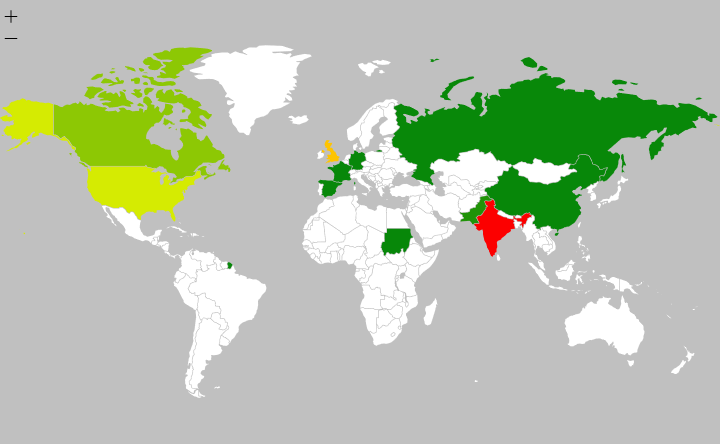
\includegraphics[width=3in]{figures/RitwikGeographicalDistro}
	\caption{Geographical density of Ritwiks, green being low and red being high.}
	\label{fig:ritwikgeographicaldistro}
\end{figure}
We collected a large sample size ($N = 12$) and used Hamiltonian Monte Carlo methods to simulate certain parameters that are backed by Bayesian goodness, undeniably proving that our method is rock solid. All data was analyzed with cutting edge tools\cite{Zaharia:2012:RDD:2228298.2228301, PyMC3}. The following math not only looks cool, but makes reviewers think that we did real work because math makes it look that way.
\begin{subequations}
\begin{align}
Count_i \sim Poi(\lambda),\\
\lambda \sim DiscreteUniform(0, 7e9),\\
\int_{\lambda}\pi(q)f(q)\sum{\frac{Var_\pi[f]}{ESS}}
\end{align}
\end{subequations}
\vspace{1in}

\section{Popularity of Ritwik Over Time}
Though Ritwiks themselves are insanely popular\footnote{Refer to our peers.}, the name Ritwik itself has not seen widespread gain in usage throughout history. Using historical databases, we were able to reconstruct the usage of the name and use popular methods such as randomly drawing a line that looks about right to estimate the future usage of the name as well.
\begin{figure}[h]
	\centering
	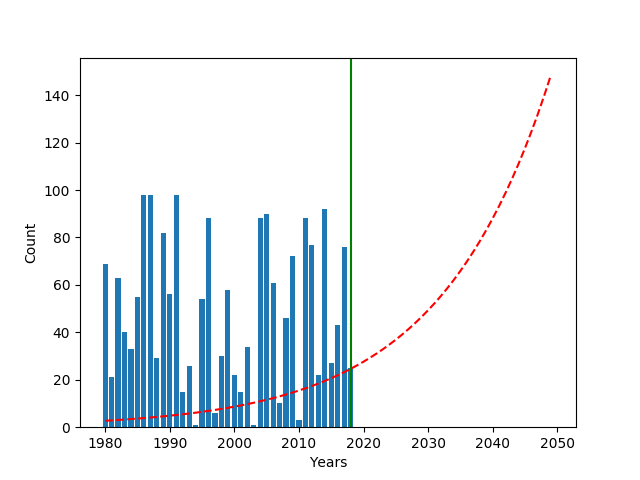
\includegraphics[width=4in]{figures/UsageOfRitwik}
	\caption{The occurrence of the name Ritwik over time. Green line represents the year this paper was published.}
	\label{fig:usageofritwik}
\end{figure}


\bibliographystyle{unsrt}
\bibliography{references}

\end{document}
